% Chapter 13: Does Nature Choose the Easiest Path?
\chapter{Does Nature Choose the Easiest Path?}

\step{A Counterintuitive Opening}

\begin{mainline}
Dip a chopstick diagonally into a glass of water and look from the side. It appears broken at the surface, as though someone bent the submerged part upward. Nobody touched it and the glass stayed still, yet you saw one straight stick become two segments. Pull it out and it is straight; put it back and it breaks again.

Now picture a beach. A lifeguard hears someone calling for help in shallow water. Dry sand and seawater separate them. She runs fast on sand but slows immediately in water. What route will she take? Almost no experienced lifeguard heads straight toward the swimmer. That route looks shortest, but spends too much distance in slow water. She runs farther diagonally along the sand, then turns into the sea. Without paper, pencil, or calculator, she chooses the quickest route.

Now comes the unsettling part. Light entering water from air also turns at the surface, in exactly the same way as the lifeguard. It seems to know that it travels faster in air and slower in water, and therefore spends more distance in air and less in water to minimize travel time. But light has neither eyes nor brain. When it starts, it has not even seen conditions at the destination. How can it choose the quickest route?

Nor is light alone. At a mirror, incidence and reflection angles are always equal, as if carefully designed. A loosely hanging clothesline looks casual, but its precise shape follows an optimizing principle. A thrown basketball's parabola hides the same secret. Does nature really choose the easiest path? If so, what does easy mean? If not, what explains these coincidences?
\end{mainline}

\step{Make a Guess First}

As usual, put your intuition on the table before peeking ahead.

First: light enters water obliquely from air. Which way does it bend? (a) Closer to the surface, almost skimming it; (b) closer to vertical, as if the water straightened it slightly; or (c) nowhere, keeping its direction.

Second: a lifeguard stands at A on a beach; a swimmer calls from B in the water. The shoreline is straight. Compare three routes: straight from A to B; farther along shore before entering almost perpendicularly; or a shorter land run followed by an early, diagonal swim. Which is fastest? What information would you need to decide?

Third: a loose rope hangs between two fixed ends. Is its shape closest to (a) a circular arc; (b) a parabola; or (c) neither? If nature likes economy, what does the rope economize: length, height, or something else?

Write down all three answers and reasons. We will check them at the end. Optics, rescue, and ropes appear unrelated; if you suspect one mechanism behind them, record that guess too. That is precisely what we are seeking.

\step{Hands-on Experiment}

\begin{experiment}[A Laser in Water: Measuring Light's Turn]
% BEGIN TRANSLATOR SAFETY NOTE
\textbf{Translator safety note:} Use the flashlight option for an unsupervised activity. Laser pointers are not toys; never aim at people or animals, and remember that reflected beams can also injure eyes. See \href{https://www.fda.gov/consumers/consumer-updates/laser-toys-how-keep-kids-safe}{FDA laser guidance}.
% END TRANSLATOR SAFETY NOTE

\textbf{Materials}: a laser pointer or bright small flashlight, a clear straight-sided glass, water, an optional drop of milk, white paper, a pen, and a protractor.

\textbf{Step 1}: fill the glass mostly with water and stir in one drop of milk to reveal the light's path. Without milk, place white paper upright behind the glass and watch the spot. Stand the glass on paper, turn off the lights, and aim the pointer along the paper obliquely at the glass wall. You will see the light bend as it enters the water, its underwater segment becoming closer to vertical.

\textbf{Step 2}: trace the paths in air and water on the paper, extend them to the entry point, and measure their angles to the perpendicular to the interface, the normal. Call them \(\theta_1\) in air and \(\theta_2\) in water. Change the angle and take three or four more readings. You will find \(\theta_2\) always smaller than \(\theta_1\), while the sine ratio \(\sin\theta_1/\sin\theta_2\) is almost constant, around \(1.3\).

\textbf{Step 3}: aim from water toward air through the glass bottom, lifting the glass and shining obliquely from below. The bending reverses: light moves away from the normal on entering air. Gradually increase the angle. Beyond a certain point, the light abruptly stops emerging and turns entirely back into the water, as though the surface became a mirror.

\textbf{Step 4, extra credit}: replace the glass with a rectangular plastic container of water, so light passes through two parallel air--water--air interfaces. Compare the outgoing and original incoming beams: their directions match exactly, but one is shifted sideways. Two parallel glass surfaces do not change light's direction, which is why the world stays undistorted through a flat window.

\textbf{Record}: note several pairs of \(\theta_1\) and \(\theta_2\). We will explain what the constant near \(1.3\) means, how it connects to least time, and how the same law produces a surface that becomes a mirror.
\end{experiment}

A free observation: at night, look at streetlit puddles, or in daylight at a straw in water. Submerged things appear shallower than they are. Put a coin in an opaque cup, step back until it just disappears, then add water. The coin floats into view. Remember your surprise.

\step{The Old Model Runs into Trouble}

Our first model says light travels straight. That works separately in air and water: both experimental segments are indeed straight. The difficulty is the interface. Why turn there, and why that way? Straight-line travel answers neither question.

So upgrade it. Two thousand years ago, Hero of Alexandria noticed something elegant: equal incidence and reflection angles are equivalent to light taking the \emph{shortest} route from source to destination via the mirror. Reflect the destination across the mirror, use the shortest straight-line distance, then unfold the construction to obtain equal angles. The old model gets a handsome patch: \emph{nature takes the shortest path}.

Unfortunately, the patch does not survive water. Refraction is not shortest-distance travel: a straight line from air to a point underwater is shortest, but light refuses it. Mechanics also rebels. A ball thrown vertically could apparently go straight to the top most quickly, yet it first moves fast and then slowly, tracing a parabola. A basketball heading for the hoop follows a curve, not a straight line. Shortest distance fails for both refraction and projectiles.

Worse, every patch invents a new thing nature cares about: distance for reflection, something else for refraction, a third thing for projectiles. That is a collection of hindsight explanations, not a theory. A deeper discomfort remains: both straightness and shortest distance describe \emph{spatial shape}, while a thrown ball crucially involves \emph{time}. It lingers high and moves quickly low down; shortest distance discards that timing entirely. We need one criterion, and first must discover what nature is economizing.

\step{Inventing New Concepts}

\begin{mainline}
\textbf{First concept: light has different speeds in different media.} This is experimental fact, not assumption. Light travels about 300,000 kilometers per second in vacuum and 225,000 in water, about three quarters as fast, and slower still in glass. Once we accept this, shortest and quickest separate. A lifeguard runs fast on sand and swims slowly, so extra distance in the fast region is worthwhile if it shortens the slow part. The same holds for light. If time is what matters, a detour through air to spend less distance in water is entirely reasonable. In the seventeenth century, Fermat made this a principle: \emph{light follows a route whose travel time is stationary among possible routes}. This is Fermat's principle.

\textbf{Second concept: compare entire paths as wholes.} This is the chapter's real conceptual upgrade. Until now, mechanics watched position, velocity, and force at the present instant, calculated the next instant, and proceeded step by step. Now we lay whole hypothetical routes from start to finish on the table, give each a total score, and ask which score is stationary. The first approach resembles driving while looking only three meters ahead; the second resembles unfolding a whole map before departure. Remarkably, both predict exactly the same motion. They are two languages for the same natural laws. Here we learn the map language.

\textbf{Third concept: stationary does not mean minimum.} The phrase easiest path can mislead us here. Imagine mountain terrain. A basin's bottom is lowest: every step raises you. That is a minimum. But a pass between peaks, a saddle point, is different. From its center, movement along the ridge raises you while movement along the valley lowers you; the first-order height change is zero in either direction. A pass is stationary too. Fermat means precisely this: \emph{slightly shift the actual path and the first-order change in total travel time is zero}. Think of the locally level footing at a pass: at its center there is no slope in any direction. Do not think of a competition where the lowest score wins. Nature does not demand least, only stationary. Indeed, certain reflected routes involving concave mirrors take the \emph{longest} time. We will revisit that counterintuitive example.

\textbf{Fourth concept: action.} Fermat covers only light. Do thrown basketballs, orbiting planets, and oscillating springs have a similar total score? Yes. Eighteenth-century physicists discovered a score for every hypothetical mechanical path, called \emph{action}, which is stationary for actual motion. Two cautions are essential. First, action is \emph{not} energy, and stationary action does not mean minimum energy. A hanging clothesline minimizes potential energy, a different principle entirely. Second, it does not mean ordinary effort or convenience. The actual path's action can be higher than nearby paths, lower, or saddle-like. Only first-order stationarity is universal. Strictly, our title's easiest should therefore be most stationary.

For an intuitive advance on the formula in the mathematical bridge, action roughly adds up kinetic energy minus potential energy over the journey. Throw a ball: going straight to the highest point and lingering there makes potential energy large and kinetic energy too small, giving an extreme difference. Skimming low saves potential energy, but reaching the endpoint in the same time requires great speed and excessive kinetic energy. The actual parabola compromises: fast where appropriate, high where appropriate, making the journey's total kinetic-minus-potential account stationary. The ball is not weighing options. Only this route satisfies Newton's law at every instant.
\end{mainline}

\begin{center}
\begin{tikzpicture}[scale=1.0]
  % Actual and perturbed paths
  \fill (0,0) circle (2pt) node[left=3pt] {Start};
  \fill (8,2.2) circle (2pt) node[right=3pt] {End};
  \draw[very thick,blue!70!black] (0,0) .. controls (2,1.6) and (5,2.4) .. (8,2.2)
    node[midway,above=6pt] {Actual path: stationary action};
  \draw[thick,dashed,red!70!black] (0,0) .. controls (2,0.2) and (5,0.6) .. (8,2.2)
    node[midway,below=8pt] {Slightly altered hypothetical path};
  \draw[-{Stealth[length=2.5mm]},gray!70!black] (3.1,1.85) -- (3.1,0.75);
  \node[gray!70!black,right=2pt] at (3.3,1.3) {Small shift};
\end{tikzpicture}
\end{center}

The idea of variation lies in that small shift. Take the actual path, nudge it slightly in any direction without moving its endpoints, and calculate the score's change. If the first-order change always vanishes, this is nature's path. First-order is crucial: shifting a millimeter does not give exactly zero change. The part \emph{proportional} to that millimeter vanishes, leaving terms proportional to its square, cube, and so on. At a mountain pass, the height change grows with step length squared, so smaller steps reveal flatter ground. The mathematical bridge will express this precisely.

A brief history prevents the impression that this idea fell from the sky. In the seventeenth century, Fermat proposed least time for light. In the eighteenth, Maupertuis conjectured an optimizing quantity for forces and named it action; Euler supplied rigorous mathematics. Lagrange and Hamilton later forged two complete mechanical languages, the subjects of Chapters 14 and 15. The traditional name stuck. Whenever a textbook says principle of least action, it means our old friend stationary action.

\step{The Model in One Sentence}

\begin{oneline}
Nature neither takes shortcuts nor chooses: actual motion follows a path whose cost, travel time for light or action for mechanics, is unchanged to first order by a small shift; it is stationary, not necessarily minimal.
\end{oneline}

\step{The Mathematical Translator}

\begin{mainline}
First calculate the lifeguard's route with realistic numbers. The shoreline is straight; the lifeguard stands at A on shore, while the swimmer is \(30\) meters offshore and \(40\) meters away along shore.

\begin{center}
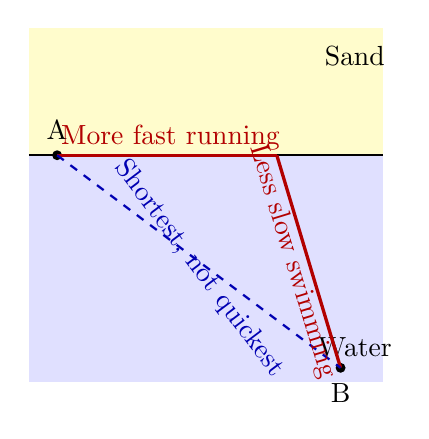
\begin{tikzpicture}[scale=0.09]
  % Shore: sand above, water below
  \fill[yellow!20] (0,0) rectangle (50,18);
  \fill[blue!12] (0,0) rectangle (50,-32);
  \draw[thick] (0,0) -- (50,0) node[midway,above=2pt] {};
  \node at (46,14) {Sand};
  \node at (46,-27) {Water};
  % A: lifeguard on shore; B: swimmer
  \fill (4,0) circle (0.7) node[above=2pt] {A};
  \fill (44,-30) circle (0.7) node[below=2pt] {B};
  % Optimal route: run about 31 meters before entering water
  \draw[very thick,red!70!black] (4,0) -- (35,0);
  \draw[very thick,red!70!black] (35,0) -- (44,-30);
  % Straight route
  \draw[thick,dashed,blue!70!black] (4,0) -- (44,-30);
  % Labels
  \node[red!70!black] at (20,2.5) {More fast running};
  \node[red!70!black,rotate=-73] at (37.2,-15) {Less slow swimming};
  \node[blue!70!black,rotate=-53] at (24,-16) {Shortest, not quickest};
\end{tikzpicture}
\end{center}

She runs at \(5\) meters per second and swims at \(1.5\) meters per second. After running \(x\) meters from A, she enters the water and swims straight to the swimmer. Total time is
\[
  T(x)=\frac{x}{5}+\frac{\sqrt{30^2+(40-x)^2}}{1.5}\ \text{s}.
\]
Compare routes. Going straight, \(x=0\), means entering immediately, with zero running time and a swim of \(\sqrt{30^2+40^2}=50\) meters: \(T=50/1.5\approx 33.3\) seconds. Running the full \(40\) meters before swimming perpendicularly gives \(T=8+30/1.5=28\) seconds, already over five seconds quicker. Try finer choices of \(x\): at \(x=25\) meters, \(T\approx27.4\) seconds; at \(x=27\), about \(27.2\); at \(x=29\), about \(27.1\); at \(x=31\), about \(27.08\); at \(x=33\), about \(27.1\); and at \(x=35\), about \(27.3\). The minimum lies near \(x\approx31\) meters, about six seconds faster than going straight. For a drowning person, six seconds can mean life or death.

Notice one feature of these numbers. Near the optimum, changing \(x\) by a full two meters changes time by only a few hundredths of a second. Farther away, the same shift changes time appreciably more. This is numerical first-order stationarity: \emph{a valley's bottom must be flat}. Conversely, finding the place barely changed by any small shift is finding the minimum here. That is how variation works: seek the stationary location instead of explicitly calculating a minimum. Notice the structure: travel about \(31\) extra meters in the fast medium to reduce the slow-medium distance from \(50\) to about \(31\) meters. \emph{Trade slow distance for fast distance}: that is refraction's whole secret.

Generalizing this trade gives the refraction law. Light travels at \(v_1\) and \(v_2\) in two media, with incidence and refraction angles \(\theta_1\) and \(\theta_2\), measured from the normal. Stationary total travel time requires
\[
  \frac{\sin\theta_1}{\sin\theta_2}=\frac{v_1}{v_2}.
\]
Write the vacuum speed as \(c\), and each medium's slowness as \(n=c/v\), its refractive index. The equation becomes symmetric:
\[
  n_1\sin\theta_1=n_2\sin\theta_2.
\]
This is Snell's law. Four questions: what does it describe? The bend at an interface. Why this form? Only this relation makes the first-order travel-time change vanish; equal sides mean shifting the entry point no longer saves time. When does it hold? At a flat interface between uniform media, with wavelength much smaller than the interface scale. When does it fail? Structures comparable to a wavelength, such as diffraction gratings and the structures producing soap-bubble colors, undermine the single-path picture and require wave optics.

Three routine checks. First, \(n_1=n_2\), the same medium on both sides, gives \(\theta_1=\theta_2\): no bend, recovering straight-line travel. Second, enormous \(n_2\), meaning extremely slow light, forces \(\sin\theta_2\) tiny. Light travels almost normally, minimizing the slow section, just like the lifeguard's perpendicular-entry limit. Third, reverse the direction from water to air: the relative sizes of \(\theta\) reverse, and the formula still holds. Optical paths are reversible, as Step 3 showed.
\end{mainline}

Now the surface that becomes a mirror. From water, \(n_1\approx1.33\), to air, \(n_2\approx1\), Snell gives \(\sin\theta_2=1.33\sin\theta_1\). As \(\theta_1\) reaches about \(49^{\circ}\), the right side reaches \(1\): \(\theta_2=90^{\circ}\), and refracted light skims the surface. Increase incidence further and the equation demands \(\sin\theta_2>1\), with no solution. Mathematical impossibility becomes total internal reflection: all the light returns into the water. Looking up, a diver sees only a bright circular window overhead, with a mirror outside it: Snell's window. Optical fibers use the same effect to confine light in thin glass strands and guide it around bends over kilometers.

A real-data estimate shows how tangible slower light is in engineering. Its effective speed in fiber is about 200,000 kilometers per second. For a 1,300-kilometer Beijing--Shanghai fiber, one-way delay is \(1300/200000\) seconds, or \(6.5\) milliseconds; round-trip delay is about \(13\) milliseconds. This is the unavoidable part of interprovincial gaming latency. Faster switches and better software cannot beat the floor set by light in glass. On another scale, three millimeters of window glass adds about \((1.5-1)\times 0.003/(3\times10^{8})\) seconds over vacuum, five picoseconds, each a trillionth of a second. Absurdly short though it seems, precision optics and atomic-clock timing must track every such entry.

\begin{mathbridge}
The mechanical score is written as follows. For mass \(m\), kinetic energy \(T=\frac12 mv^2\), and potential energy \(V\), both familiar from Chapter 9, define the action of each hypothetical path \(x(t)\) as
\[
  S[\,x(t)\,]=\int_{t_1}^{t_2}\bigl(T-V\bigr)\,dt,
\]
adding kinetic minus potential energy at every instant of the journey. The actual path satisfies
\[
  \delta S=0,
\]
meaning that if the path becomes \(x(t)+\varepsilon\,\eta(t)\), with arbitrary perturbation \(\eta\) vanishing at both ends and infinitesimal \(\varepsilon\), the change in \(S\) has zero first-order term in \(\varepsilon\). Notice the minus sign in \(T-V\). This is not total energy \(T+V\), so stationary action never means minimum energy.

Why is this equivalent to Newton's law? Intuitively, shift a short portion of the path upward. The potential-energy integral \(V\) changes because position changes, while the kinetic-energy integral \(T\) changes through velocity. To make the first-order total vanish, these effects must cancel exactly. Written point by point, the cancellation condition is \(F=ma\). Least action is therefore not a second natural law beside Newton's. They are two faces of one coin: Newton speaks locally at each instant; action speaks globally over a journey. Each translates exactly into the other.

Compare light's version: Fermat adds the travel times \(n\,ds/c\) of tiny segments, whereas action adds \(T-V\) at successive instants. Two chapters from now, Chapter 15 will place even these different accumulated quantities within a more general framework.
\end{mathbridge}

\begin{challenge}
Stationary rather than minimum means zero first variation. Expand \(S[x+\varepsilon\eta]\) in \(\varepsilon\) and require the first-order term to vanish for every \(\eta(t)\). This yields a differential equation valid at every point, Euler's equation. Chapter 14 follows this route to build Lagrangian mechanics.

Here is a seed for the distant future. Feynman later gave a quantum answer to how light knows the quickest route: it does not know, and it does not take only one route. Quantum descriptions include \emph{all} paths from start to finish. Each contributes an amplitude with a phase determined by action. Near a stationary path, neighboring actions and phases are nearly equal, so amplitudes reinforce. Far away, phases vary wildly and cancel. The macroscopic appearance of light choosing a stationary path is the survivor of a collective vote by countless paths. This story begins properly after Chapter 42. For now, remember that stationarity will outlive Newton's law: it still holds in the quantum world, where Newton's law does not.
\end{challenge}

\step{The Model's Limits}

\begin{mainline}
First pin down the territory, then inventory misuses.

Fermat's principle requires uniform or slowly varying media and interface scales much larger than wavelength. In graded media, paths curve continuously, as in mirages. Wavelength-scale structures causing diffraction and nonlinear media under intense light require other theories.

The action principle requires forces expressible through potential energy, as gravity, elasticity, and electrostatics can be; otherwise the standard framework cannot accommodate them. Dissipative friction is troublesome. Where energy goes when you rub your hands warm requires thermodynamics; the action principle alone cannot explain it. It is not wrong, but cannot handle that dissipative account. Another hidden condition: fix the endpoints, including their times, before comparing paths. Asking for the stationary route from home to work is meaningful; asking for the stationary route to anywhere is not a defined problem.
\end{mainline}

Typical misuses:

\begin{itemize}[leftmargin=1.8em]
  \item \emph{``Nature has a purpose: it wants to be lazy.''} That is personification, not experimental fact. The fact is equivalence between stationarity and equations of motion; anything further is literature. The causal direction is opposite: nature does not survey the whole route and choose. Local laws hold at every instant, and their combined effect makes the whole path stationary. Ant colonies likewise produce efficient routes without a global planner. Macroscopic wisdom emerges from microscopic rules.
  \item \emph{``Least action means least energy.''} Entirely different. The accumulated quantity is \(T-V\), not \(T+V\); actual action can even be \emph{larger} than that of nearby paths. For minimum energy, consult a hanging clothesline, whose static equilibrium minimizes potential energy, not action.
  \item \emph{``The principle of shortest time.''} The name is already half wrong. Some concave-mirror paths take the \emph{longest} time, and some legitimate detouring plane-mirror paths are saddles. The rigorous term is always stationary. Mentally replace every least-action principle with stationary-action principle and avoid the trap.
  \item \emph{``If global and local languages are equivalent, we no longer need Newton's laws.''} No. The global language excels at heavily constrained problems, Chapter 14's territory. Force analysis and the instantaneous details of contact and collisions still require force and acceleration. The languages support rather than replace each other.
\end{itemize}

\step{Explaining the Opening Phenomenon}

Now check the accounts, beginning with your predictions.

First: entering water from air gives \(\theta_2<\theta_1\), closer to vertical, answer b. Your measurements and the ratio near \(1.3\), water's refractive index, confirm it.

Second: the lifeguard's route depends on the speed ratio. Faster running and slower swimming favor more distance along shore. At \(5\) versus \(1.5\) meters per second, our optimum saves about six seconds over a straight route. This is light's account with a speed ratio in place of refractive index.

Third: the clothesline is neither circular nor parabolic, but a catenary. It only approximates a parabola when fairly taut with little sag. It economizes gravitational potential energy: among hypothetical shapes with fixed endpoints and length, the actual shape puts the whole rope's center of mass lowest. Moving any point up or down raises total potential energy. This is stationary, minimum potential energy rather than least action, but the reasoning has the same structure: compare a whole curve, shift it slightly, and demand first-order stationarity. Spiderwebs, high-voltage transmission lines, and suspension-bridge main cables are engineering relatives. Bridge designers hang the deck load and let the cable find its stationary shape, so the material carries tension rather than resisting bending moments.

One mirror remains unaccounted for. Why are incidence and reflection angles equal? Fermat settles it: in a uniform medium speed is constant, so least time means shortest distance. The shortest route via the mirror occurs at equal angles, which Challenge 1 asks you to prove. Reflection, refraction, projectiles, and ropes now share the phrase: shift slightly, and the first-order change vanishes.

The chopstick breaks because light leaving it bends away from the normal as it crosses into air, obeying Snell. Your eyes trace the rays backward in straight lines and locate the submerged part higher and shallower. Pools appearing roughly a quarter shallower and a hidden coin reappearing after water is added share this account. A mirage is the graded version: hot air near a road has a slightly lower refractive index. Light continually trades slow distance for fast distance through successive layers, curves upward, and brings sky light into your eyes, resembling a pool.

Quieter applications sit on your face and in your pocket: eyeglasses, camera lenses, and telescopes. Lens designers use glass of different shapes and refractive indices to redistribute segment-by-segment travel times. Rays from one object point passing through different lens regions must take equal times to the image point. Equally stationary paths then converge sharply. Miscalculate one curvature and a path arrives early or late, blurring the image. Your phone's tiny camera contains five or six oddly shaped lens elements, each solving this stationarity problem.

So does nature choose the easiest path? It neither chooses nor pursues ease. There is simply a path indifferent to a small shift. Equal reflection angles, a constant refraction ratio, and curved projectile paths all grow from that statement.

\step{Thought Experiments and Challenges}

\begin{thought}[Cover Half the Sun: Is Light's Path Still Stationary at Extreme Scales?]
During a total eclipse, starlight grazes the Sun on its way to Earth. Newtonian intuition suggests a straight path, yet observations show a small, definite gravitational bend. General relativity in Chapter 41 offers a strikingly similar interpretation: light still follows a stationary path, but mass curves spacetime near the Sun, so stationarity must be measured with curved-spacetime rulers. The path is a geodesic, as straight as possible in a curved world. Our map language survives extreme scales and becomes gravity's own theory. Planets orbit by freely sliding along spacetime geodesics, with no central string pulling them. A question about light bending ultimately incorporates gravity itself.

You have already seen stationary routes in a curved world from an airliner. A Beijing--New York route bends northward toward the Arctic on a flat map, apparently detouring. But Earth is spherical and the map flattened; the sphere's straightest route looks curved when projected onto paper. Airlines choose it for shortest distance and fuel economy, not scenery. Spherical geodesics, starlight near the Sun, and a hanging catenary share a sentence structure: define the right measure of stationarity, then apply a small variation.
\end{thought}

\begin{thought}[What If Light Really Takes Every Path?]
Water the seed from the challenge section. Put a single-slit screen between a light source and a viewing screen. As the slit narrows, Fermat still suggests one ray. But once the width approaches a wavelength, experiments show a spread-out diffraction pattern: the single-path picture fails. The quantum answer is that light always takes every path. At macroscopic scales, paths away from stationarity cancel completely. A narrow slit removes most paths, preventing clean cancellation among those remaining and exposing the stationary path's apparent monopoly. The important point: microscopic physics does not overthrow this chapter's principle but elevates it. Action changes from a computational shortcut into an entrance ticket to quantum theory, beginning in Chapter 42.
\end{thought}

\begin{puzzles}
\item Derive reflection from Fermat: light travels from A to B via a plane mirror. Show that the least-time, here also shortest-distance, route has equal incidence and reflection angles. \emph{Hint}: reflect B behind the mirror to image point B$'$. The distance from A via any mirror point to B equals that via the same point to B$'$. What is the shortest route from A to B$'$? A straight line. What relation do its angles make where it meets the mirror?
\item Why does a diver looking upward see a circular bright window surrounded by a dark, shiny mirror? Estimate its half-angle. \emph{Hint}: use Snell's law \(n_1\sin\theta_1=n_2\sin\theta_2\) from water to air. Set \(\theta_2=90^{\circ}\), substitute \(n_1\approx1.33\) and \(n_2\approx1\), and find the critical angle, about \(49^{\circ}\). More oblique light undergoes total internal reflection and cannot reach the eye.
\item Two playground slides begin at the same height and end at the same low point. One is straight; the other drops steeply, dips, then finishes gently. Which arrives first? Is shortest therefore fastest? \emph{Hint}: that distinction is this chapter's core. The curve converts height into speed early, raising average speed enough to win despite extra distance; the limiting problem is the brachistochrone. Could an excessively deep or flat curve instead be slower? Where is the stationary compromise?
\item A visitor sees a tree across a lake and its inverted reflection. Light from its top takes both a direct route to the eye and a reflected route via water. Both exist. Does Fermat not allow only one? \emph{Hint}: there can be several stationary values, like several mountain passes. Direct and reflected paths each have zero first-order change under small shifts, and nature uses both. This also explains mirror images: every ray solves its own stationarity problem.
\end{puzzles}

We now have a new language. Instead of asking at each instant where motion goes next, unfold the entire path and ask which is stationary. It works for refraction, reflection, projectiles, and clotheslines, but its real power remains ahead. Next chapter, accumulate \(T-V\), vary the path slightly, and \(F=ma\) emerges from stationarity on its own. Rotating, constrained, and many-degree-of-freedom systems that trouble Newton's language become surprisingly simple. That is Lagrangian mechanics.
